\documentclass[../../main.tex]{subfiles}
\graphicspath{{\subfix{../../images/}}}

\begin{document}

Warum nehmen wir die Farbe einer roten Paprika als "rot" wahr? Erkläre mit wenigen Worten und zeichne eine beispielhafte Kurve in den unten stehenden Graph.

\begin{figure}[h]
    \centering
    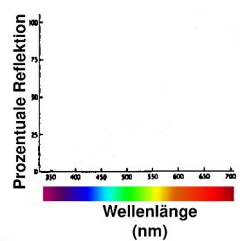
\includegraphics[width=0.75\textwidth]{tomate}
    \caption{Prozentuale Reflektion vs Wellenlänge}
    \label{fig:tomate}
\end{figure}

\end{document}


